
%--------------------------------------------------------------------
%--------------------------------------------------------------------
% Formato para los talleres del curso de Métodos Computacionales
% Universidad de los Andes
% 2015-10
%--------------------------------------------------------------------
%--------------------------------------------------------------------

\documentclass[11pt,letterpaper]{exam}
\usepackage[utf8]{inputenc}
\usepackage[spanish]{babel}
\usepackage{graphicx}
\usepackage{mdframed}
\usepackage{tabularx}
\usepackage[absolute]{textpos} % Para poner una imagen completa en la portada
\usepackage{multirow}
\mdfdefinestyle{mystyle}{leftmargin=1cm,rightmargin=1cm,linecolor=red}
\usepackage{float}
\usepackage{hyperref}
\usepackage{amsmath}
\decimalpoint
%\usepackage{pst-barcode}
%\usepackage{auto-pst-pdf}

\newcommand{\base}[1]{\underline{\hspace{#1}}}
\boxedpoints
\pointname{ pt}
%\extrawidth{0.75in}
%\extrafootheight{-0.5in}
\extraheadheight{-0.15in}
%\pagestyle{head}

%\noprintanswers
%\printanswers
\renewcommand{\solutiontitle}{}
\SolutionEmphasis{\color{blue}}

\usepackage{upquote,textcomp}
\newcommand\upquote[1]{\textquotesingle#1\textquotesingle} % To fix straight quotes in verbatim

\begin{document}
\begin{center}
{\Large Métodos Computacionales} \\
Taller 6 - \textsc{Ecuaciones diferenciles ordinarias y parciales} \\
Profesor: Sebastián Pérez Saaibi\\
Fecha de Publicación: {\small \it Marzo 23 de 2015}\\
\end{center}

\begin{textblock*}{40mm}(10mm,20mm)
  
\includegraphics[width=3cm]{logoUniandes.png}
\end{textblock*}

\begin{textblock*}{40mm}(161mm,20mm)
  
\includegraphics[width=3cm]{logoUniandes.png}
\end{textblock*}

\vspace{0.5cm}

{\Large Fecha de Entrega:  \bf Abril 22 de 2015 antes de las 23:59 COT}

\vspace{0.5cm}

{\Large Instrucciones de Entrega}\\

Todo el código fuente y los datos se debe encontrar en un repositorio público en github con un commit final hecho antes de la fecha de entrega. El nombre del repositorio debe ser \newline \verb+CM20151_HW6_Apellido1Apellido2+. El link al repositorio lo deben enviar a través de \textbf{sicuaplus} antes de la fecha/hora límite. Se hará una entrega parcial de discusión de progreso el Jueves 16 de Abril 07:00 COT. Esa entrega entrega parcial es obligatoria para que su taller tenga nota distinta de cero.

En cada parte del ejercicio se entrega 1/3 de los puntos si el código propuesto es razonable, 1/3 si se puede ejecutar y 1/3 si entrega resultados correctos.


\vspace{0.5cm}

\begin{questions}

\question[50] {\bf El fin del mundo?}

Se ha descubierto un supuesto asteroide que al parecer va a pasar por la tierra, la NASA ha contratado a los estudiantes de Métodos Computacionales para que encuentren la orbita de dicho asteroide y determinen si realmente constituye un peligro para la tierra. Para esto hay que resolver la ecuación gravitacional: 
 
\begin{equation}\label{eq:force}
\dfrac{d^2\vec{r_i}}{dt^2} = \sum_{j=1, j!=i}^{N} \dfrac{Gm_j (r_i-r_j)}{|\vec{r_i}-\vec{r_j}|^3}
\end{equation}   

Considere el sistema \textbf{Tierra-Sol-Luna-Asteroide}, con las siguientes condiciones iniciales:

\begin{itemize}

\item $x_{sol}=y_{sol}=z_{sol}=0$

\item $x_{tierra} = 1, y_{tierra}=z_{tierra}=0$

\item $x_{luna} = 1.0026, y_{luna}=0, z_{luna}=0$

\item $x_{ast} = 1, y_{ast}=0.0963, z_{ast}=0$

\item $Vx_{sol}=Vy_{sol}=Vz_{sol}=0$

\item $Vx_{tierra} = 0, Vy_{tierra}=30 km/s, Vz_{tierra}=0$

\item $Vx_{luna} = 0, Vy_{luna}=1.023 km/s, Vz_{luna}=0$

\item $Vx_{ast} = 1570 km/s, Vy_{ast}=0, Vz_{ast}=29959 km/s$

\item $M_{sol} = 1$, $M_{tierra}=3.003E-6$, $M_{luna}=3.695E-8$, $M_{ast} = 5E-11$
\end{itemize}


\begin{parts}
\part[30] Escriba un codigo en C (\verb+4body.c+) que resuelva la ecuaci\'on \ref{eq:force} usando Runge-kutta4 teniendo en cuenta las condiciones iniciales. El codigo debe leer un archivo con las condiciones iniciales $ic.txt$. Adicionalmente el codigo debe compilarse as\'i:
 
\verb+./4body.x ic.txt h t+  

Donde $h=x - x_0$ y $t = N/h$ es el tiempo, ajuste $N$ de tal forma que la tierra de una orbita completa alrededor del Sol. El codigo debe escribir un archivo \verb+orbitas.txt+ con las orbitas del Sol, Tierra, Luna, Asteroide en coordenadas cartesianas. Haga esto para dos tiempos diferentes $t_1 = 1$ año terrestre y $t_2=1000$ años terrestres. 

\part[10] Escriba un codigo en python \verb+treyectorias.py+ que lea el archivo \verb+orbitas.txt+ y haga graficas en el plano (X, Y) de las orbitas, este programa debe generar dos figuras $orbitas-1yr.png$ y $orbitas-1000yr.png$ correspondientes a los tiempos $t_1$ y $t_2$.

\part[10] Escriba un Makefile que compile y ejecute todos los programas.
\end{parts}


\question[50] {\bf Difusión en un reactor tubular}

Un fluído newtoniano se mueve dentro de un reactor químico tubular con flujo laminar, de la siguiente manera:

\begin{figure}[H]
\centering
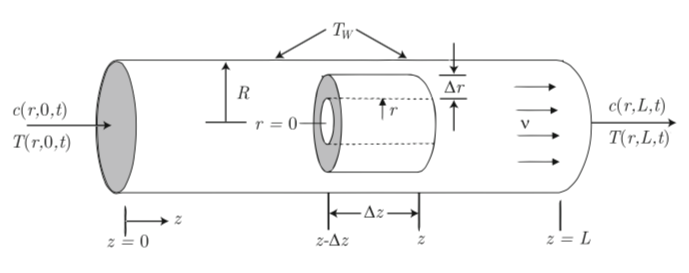
\includegraphics[width=0.8\textwidth]{tubular_reactor.png}
\caption{Reactor Tubular}
\end{figure}

En dos dimensiones el problema del reactor se puede plantear con sus respectivos balances de masa y energía, incluyendo convección, difusión y una reacción química.

Se puede expresar de la siguiente manera
\begin{align*}
	c_t = -v(r)c_z + D(c_{zz} + c_{rr} + \frac{1}{r}c_r ) -r(c,T) \\
	T_t = -v(r)T_z + \frac{\lambda}{\rho c_{p}}(T_{zz} + T_{rr} + \frac{1}{r}T_r ) + \frac{- \Delta H}{\rho c_{p}}r(c,T)
\end{align*}

Donde $r(c,T) = k_0 \exp(-\frac{E}{RT})c^2$.
El perfil de velocidad de flujo parabólico corresponde a $v(r) = v_{max} (1 - (\frac{r}{R})^2)$.

Las \textbf{condiciones iniciales} son:
\begin{align*}
	c(r,z,0) = c_0(r,z) \\
	T(r,z,0) = T_0(r,z)
\end{align*}

Las \textbf{condiciones de frontera} son:

Simetría Radial sin transferencia de masa 
\begin{align*}
	c_r(0,z,t) = 0 \\
	T_r(0,z,t) = 0 \\
	c_r(R,z,t) = 0
\end{align*}

Intercambio térmico con la pared
\begin{align*}
	T_r(R,z,t) = \frac{h}{\lambda}(T_w -T(R,z,t))
\end{align*}

Concentración y Temperatura constantes al interior del tubo

\begin{align*}
	c(r,0,t) = c_{in} \\
	T(r,0,t) = T_{in}
\end{align*}

Difusión cero a la salida
\begin{align*}
	c_z(r,L,t) = 0 \\
	T_z(r,L,t) = 0
\end{align*}

\begin{parts}
\part[5] Usando la regla de l'Hôpital, muestre que para $r = 0$, es decir, en el centro del tubo:

\begin{align*}
	c_t = -v c_z + D(c_{zz} + 2 c_{rr}) -r(c,T) \\
	T_t = -v T_z + \frac{\lambda}{\rho c_{p}}(T_{zz} + 2T_{rr} ) + \frac{- \Delta H}{\rho c_{p}}r(c,T)
\end{align*}

\part[35] Escriba un programa (en R, Python o C) que resuelva la PDE en 2D con el método de diferencias finitas. El programa debe mostrar la solución de manera gráfica para la concentración $c(r,z,t)$ y la temperatura $T(r,z,t)$. Puede usar gráficos en 3D o curvas de nivel.

\part[10] Escriba un programa que resuelva el problema en 1D (es decir, resuelva para el centro del tubo y asuma que no hay diferencias con variaciones del radio). El programa debe mostrar la solución de manera gráfica para la concentración $c(z,t)$ y la temperatura $T(z,t)$. Use curvas de nivel.

Para su solución, puede usar las siguientes especificaciones

\begin{align*}
	R = 1; L = 30; T_w = 100; k_0 = 10; E = 10
\end{align*}

\textbf{Nota}: En general, escriba sus funciones para recibir valores distintos de dichos parámetros y de otros que no están especificados claramente ($\Delta H, \rho, \lambda, h, ...$). De qué material es el reactor tubular? Cuáles son sus propiedades?Especifique sus supuestos claramente antes de la primera entrega.

\end{parts}

\end{questions}
\end{document}
